%Mastering Suite
\begin{figure}
    \centering
    \begin{subfigure}[t]{0.3\textwidth}
       \centering
       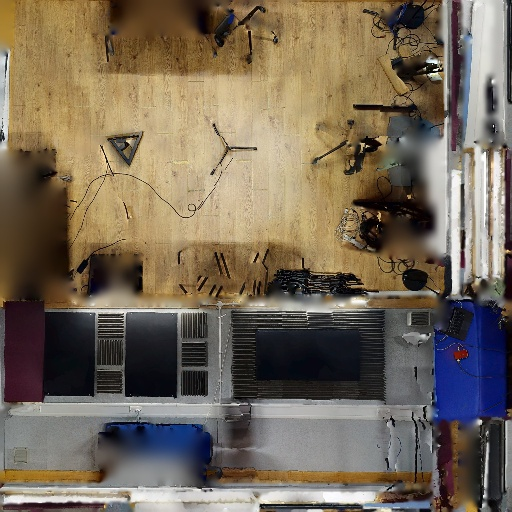
\includegraphics[width=\textwidth]{poc/t_mastering_suite_0.jpg}

    \end{subfigure}
    \begin{subfigure}[t]{0.3\textwidth}
       \centering
       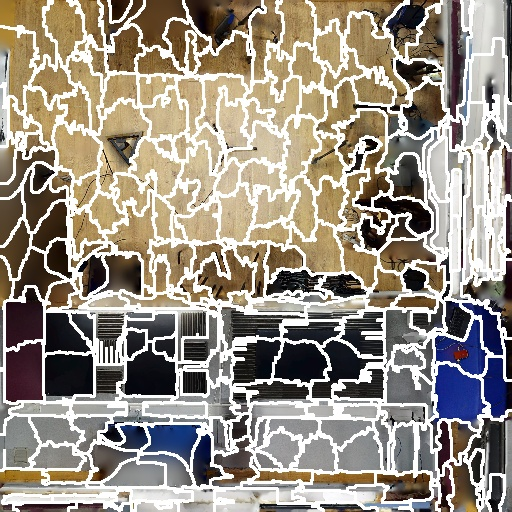
\includegraphics[width=\textwidth]{poc/x_mastering_suite_0.jpg}

    \end{subfigure}
    \begin{subfigure}[t]{0.3\textwidth}
        \centering
        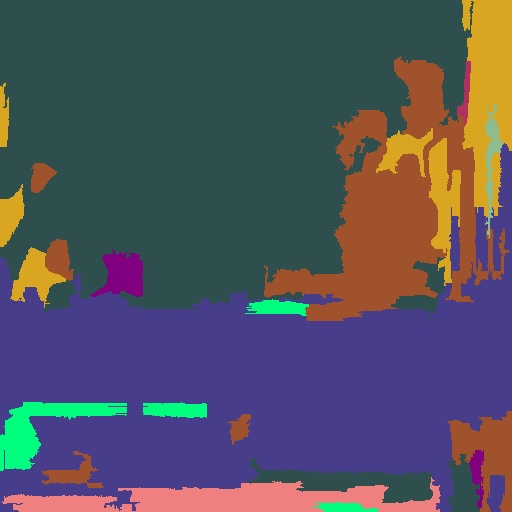
\includegraphics[width=\textwidth]{poc/s_mastering_suite_0.jpg}
     \end{subfigure}


    \addvspace{\baselineskip}


    \centering
    \begin{subfigure}[t]{0.3\textwidth}
       \centering
       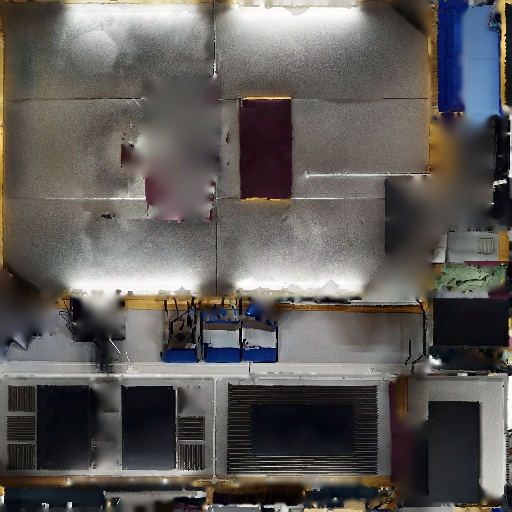
\includegraphics[width=\textwidth]{poc/t_mastering_suite_1.jpg}

    \end{subfigure}
    \begin{subfigure}[t]{0.3\textwidth}
       \centering
       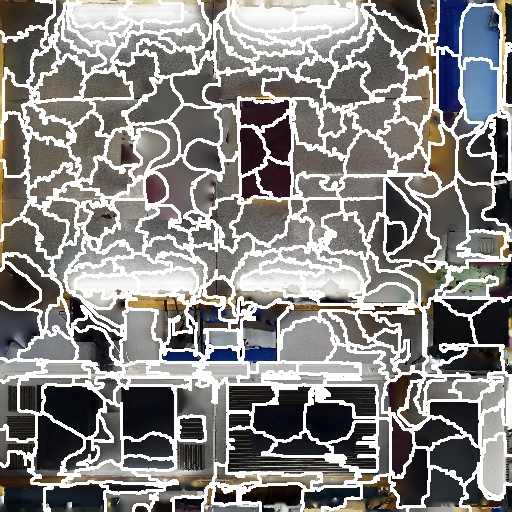
\includegraphics[width=\textwidth]{poc/x_mastering_suite_1.jpg}

    \end{subfigure}
    \begin{subfigure}[t]{0.3\textwidth}
        \centering
        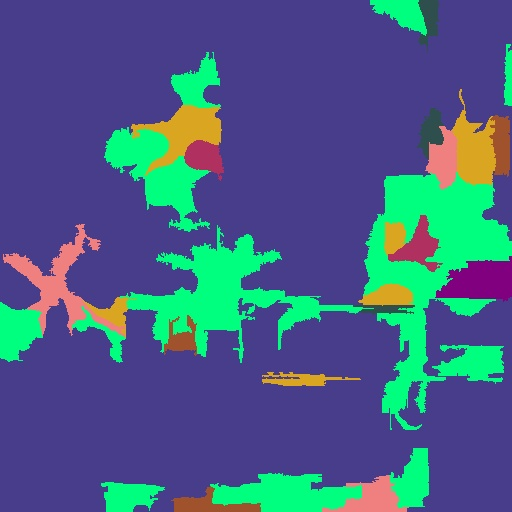
\includegraphics[width=\textwidth]{poc/s_mastering_suite_1.jpg}
     \end{subfigure}


    \addvspace{\baselineskip}

    
    \centering
    \begin{subfigure}[t]{0.3\textwidth}
       \centering
       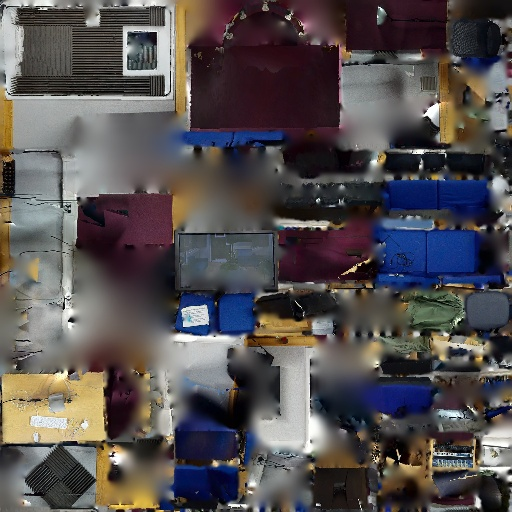
\includegraphics[width=\textwidth]{poc/t_mastering_suite_2.jpg}
       \caption{Input Texture}
    \end{subfigure}
    \begin{subfigure}[t]{0.3\textwidth}
       \centering
       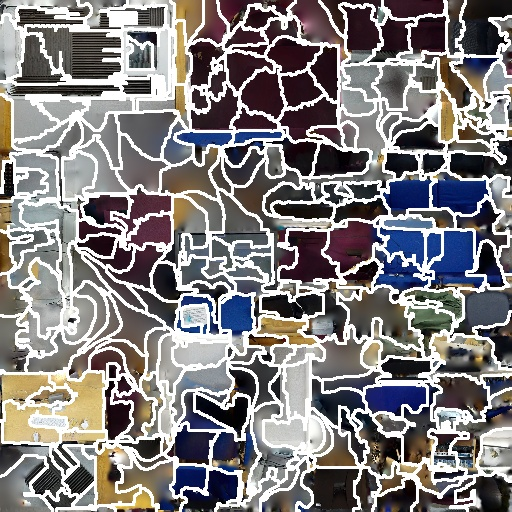
\includegraphics[width=\textwidth]{poc/x_mastering_suite_2.jpg}
       \caption{Superpixel Segmentation}
    \end{subfigure}
    \begin{subfigure}[t]{0.3\textwidth}
        \centering
        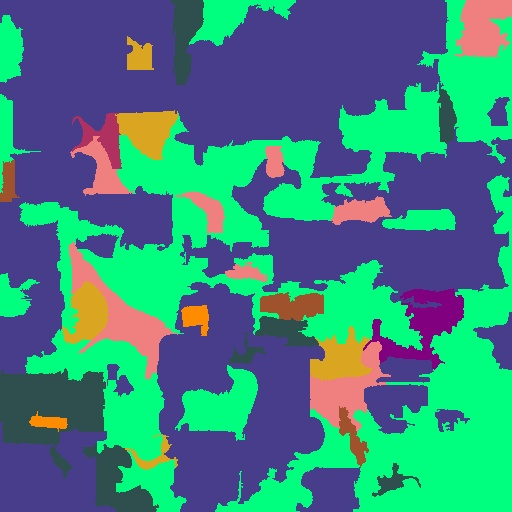
\includegraphics[width=\textwidth]{poc/s_mastering_suite_2.jpg}
        \caption{Material Tagging}
     \end{subfigure}
 

\caption{Material Tagging performed on textures from the Mastering Suite scene.}
\label{fig:mastering-suite-superpixels}
\end{figure}
%Recital Hall
\begin{figure}
    \centering
    \begin{subfigure}[t]{0.3\textwidth}
       \centering
       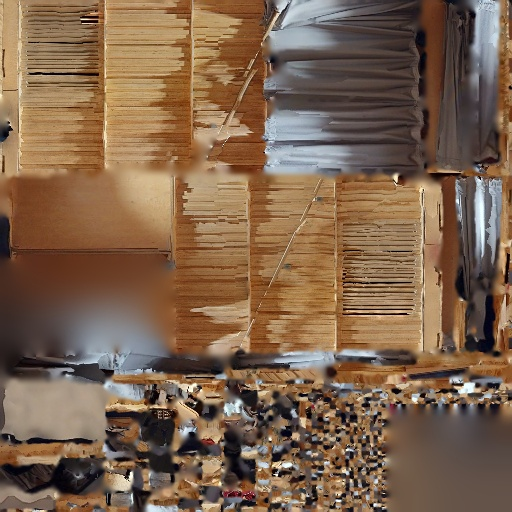
\includegraphics[width=\textwidth]{poc/t_conservatoire_0.jpg}

    \end{subfigure}
    \begin{subfigure}[t]{0.3\textwidth}
       \centering
       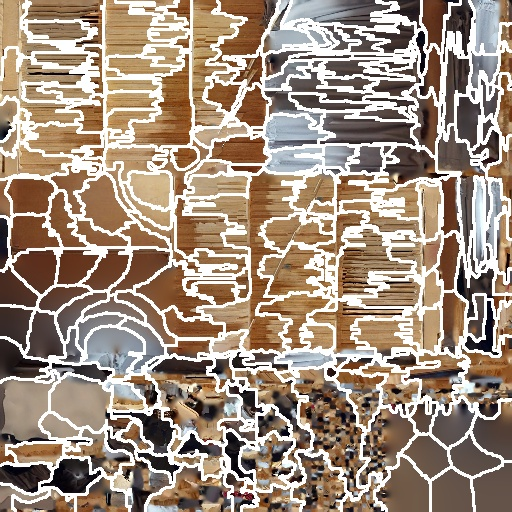
\includegraphics[width=\textwidth]{poc/x_conservatoire_0.jpg}

    \end{subfigure}
    \begin{subfigure}[t]{0.3\textwidth}
        \centering
        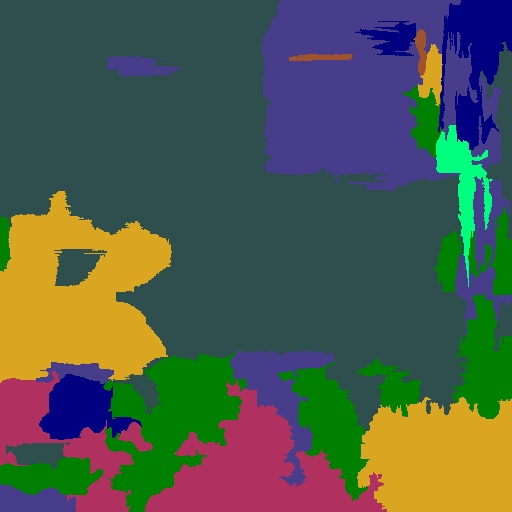
\includegraphics[width=\textwidth]{poc/s_conservatoire_0.jpg}
     \end{subfigure}


    \addvspace{\baselineskip}


    \centering
    \begin{subfigure}[t]{0.3\textwidth}
       \centering
       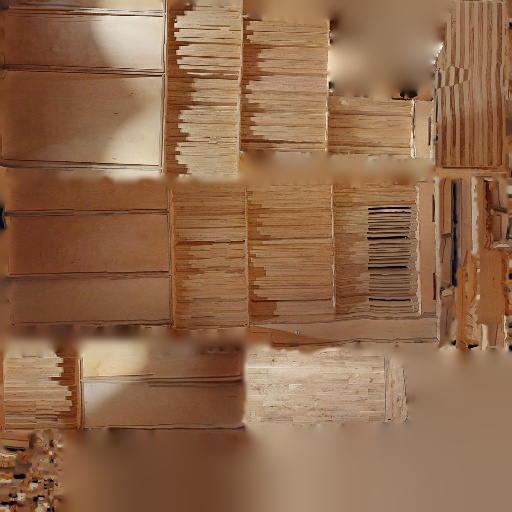
\includegraphics[width=\textwidth]{poc/t_conservatoire_1.jpg}

    \end{subfigure}
    \begin{subfigure}[t]{0.3\textwidth}
       \centering
       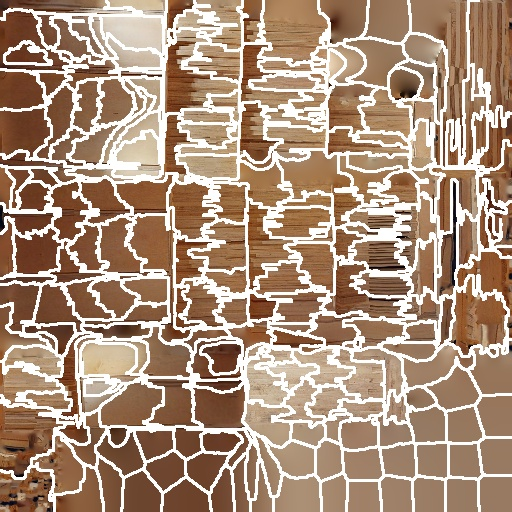
\includegraphics[width=\textwidth]{poc/x_conservatoire_1.jpg}

    \end{subfigure}
    \begin{subfigure}[t]{0.3\textwidth}
        \centering
        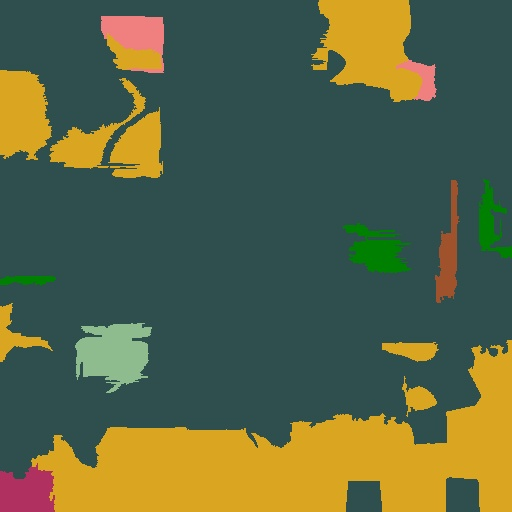
\includegraphics[width=\textwidth]{poc/s_conservatoire_1.jpg}
     \end{subfigure}


    \addvspace{\baselineskip}

    
    \centering
    \begin{subfigure}[t]{0.3\textwidth}
       \centering
       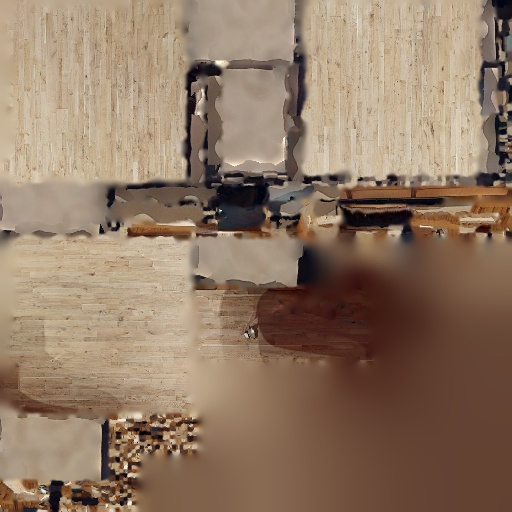
\includegraphics[width=\textwidth]{poc/t_conservatoire_2.jpg}
       \caption{Input Texture}
    \end{subfigure}
    \begin{subfigure}[t]{0.3\textwidth}
       \centering
       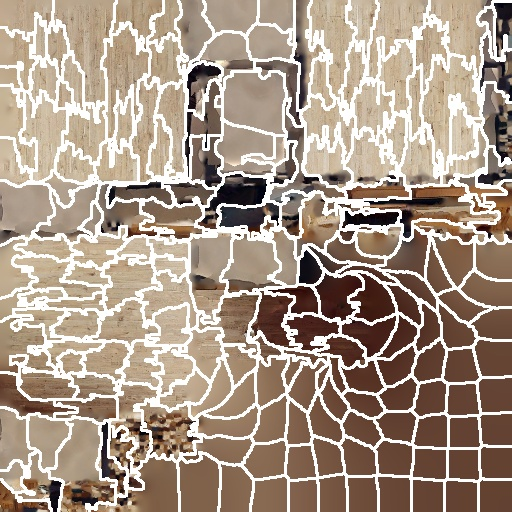
\includegraphics[width=\textwidth]{poc/x_conservatoire_2.jpg}
       \caption{Superpixel Segmentation}
    \end{subfigure}
    \begin{subfigure}[t]{0.3\textwidth}
        \centering
        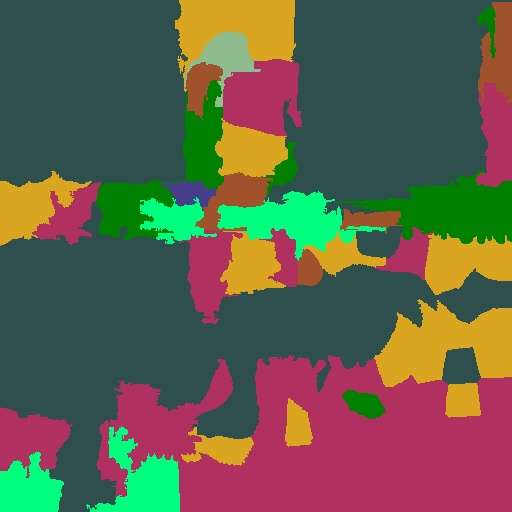
\includegraphics[width=\textwidth]{poc/s_conservatoire_2.jpg}
        \caption{Material Tagging}
     \end{subfigure}
 

\caption{Material Tagging performed on textures from the Recital Hall scene.}
\label{fig:recital-hall-superpixels}
\end{figure}
%Guild Hall
\begin{figure}
    \centering
    \begin{subfigure}[t]{0.3\textwidth}
       \centering
       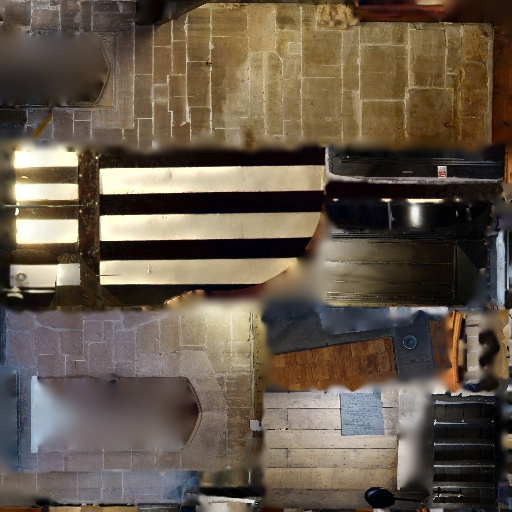
\includegraphics[width=\textwidth]{poc/t_GuildHall_0.jpg}

    \end{subfigure}
    \begin{subfigure}[t]{0.3\textwidth}
       \centering
       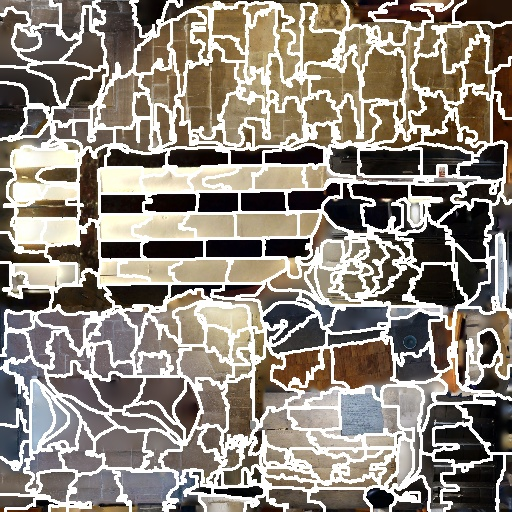
\includegraphics[width=\textwidth]{poc/x_GuildHall_0.jpg}

    \end{subfigure}
    \begin{subfigure}[t]{0.3\textwidth}
        \centering
        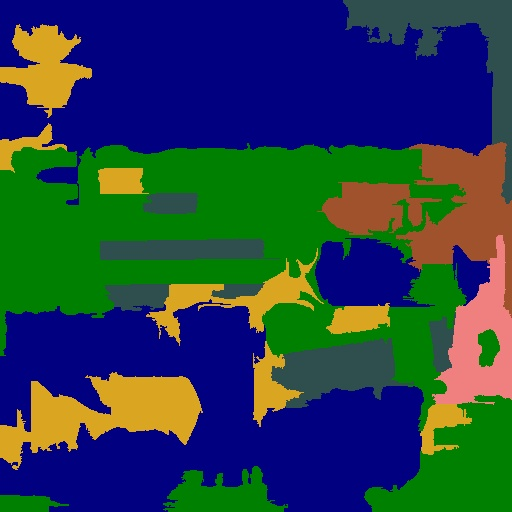
\includegraphics[width=\textwidth]{poc/s_GuildHall_0.jpg}
     \end{subfigure}


    \addvspace{\baselineskip}


    \centering
    \begin{subfigure}[t]{0.3\textwidth}
       \centering
       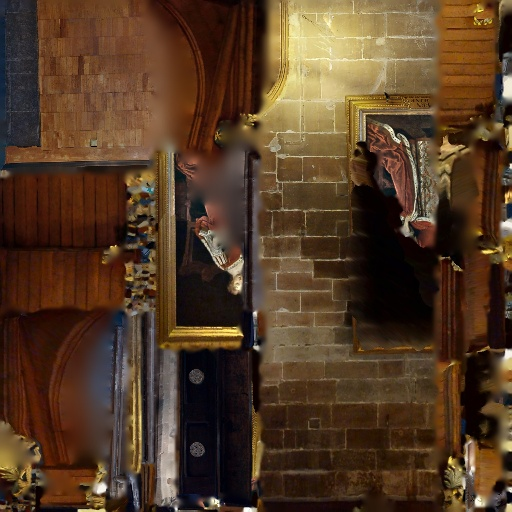
\includegraphics[width=\textwidth]{poc/t_GuildHall_1.jpg}

    \end{subfigure}
    \begin{subfigure}[t]{0.3\textwidth}
       \centering
       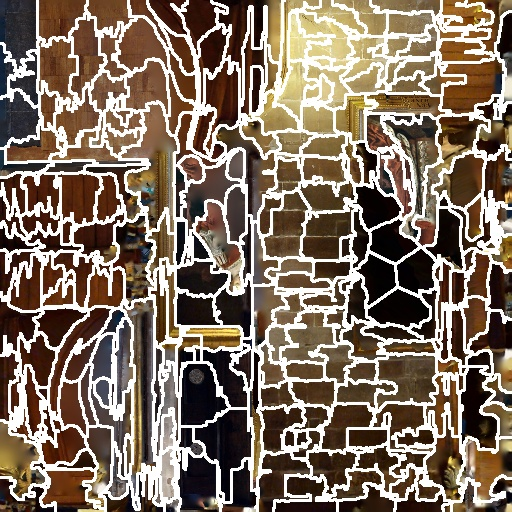
\includegraphics[width=\textwidth]{poc/x_GuildHall_1.jpg}

    \end{subfigure}
    \begin{subfigure}[t]{0.3\textwidth}
        \centering
        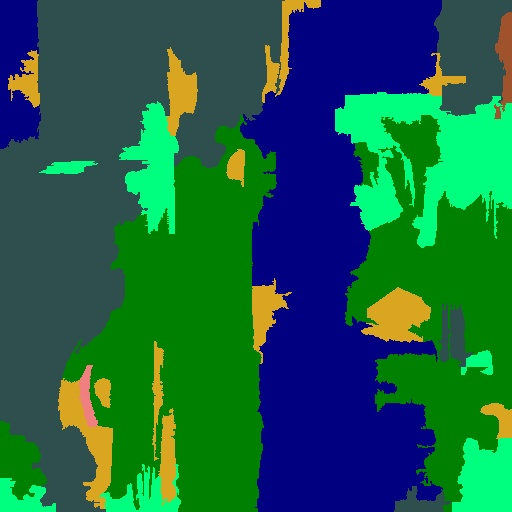
\includegraphics[width=\textwidth]{poc/s_GuildHall_1.jpg}
     \end{subfigure}


    \addvspace{\baselineskip}

    
    \centering
    \begin{subfigure}[t]{0.3\textwidth}
       \centering
       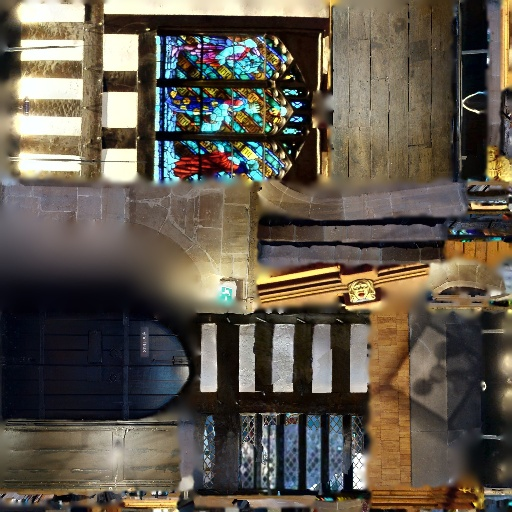
\includegraphics[width=\textwidth]{poc/t_GuildHall_2.jpg}
       \caption{Input Texture}
    \end{subfigure}
    \begin{subfigure}[t]{0.3\textwidth}
       \centering
       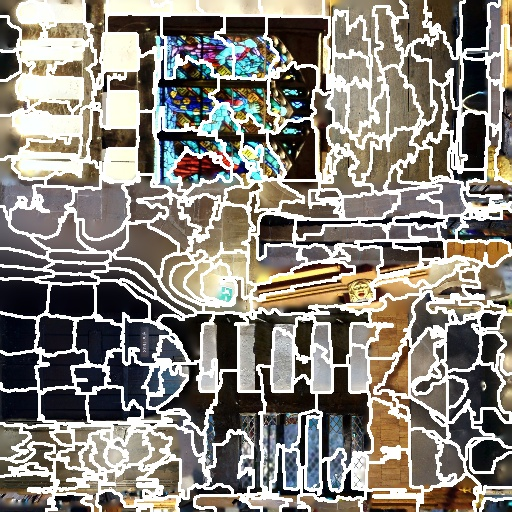
\includegraphics[width=\textwidth]{poc/x_GuildHall_2.jpg}
       \caption{Superpixel Segmentation}
    \end{subfigure}
    \begin{subfigure}[t]{0.3\textwidth}
        \centering
        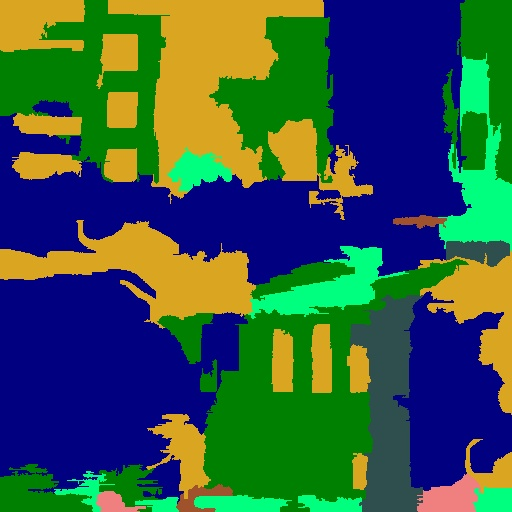
\includegraphics[width=\textwidth]{poc/s_GuildHall_2.jpg}
        \caption{Material Tagging}
     \end{subfigure}
 

\caption{Material Tagging performed on textures from the St Mary's Guild Hall scene.}
\label{fig:guild-hall-superpixels}
\end{figure}